\section{Detailed Annotation Guidelines for Challenging Cases}
\markright{Detailed Annotation Guidelines}
\label{sec:cis:supplementary-annotation-guidelines}

This section provides visual annotation guidance for challenging appearances encountered during the construction of CholecInstanceSeg.

\begingroup
\renewcommand{\thefigure}{S\arabic{figure}}
\setcounter{figure}{0}

\begin{figure}[htb!]
  \centering
  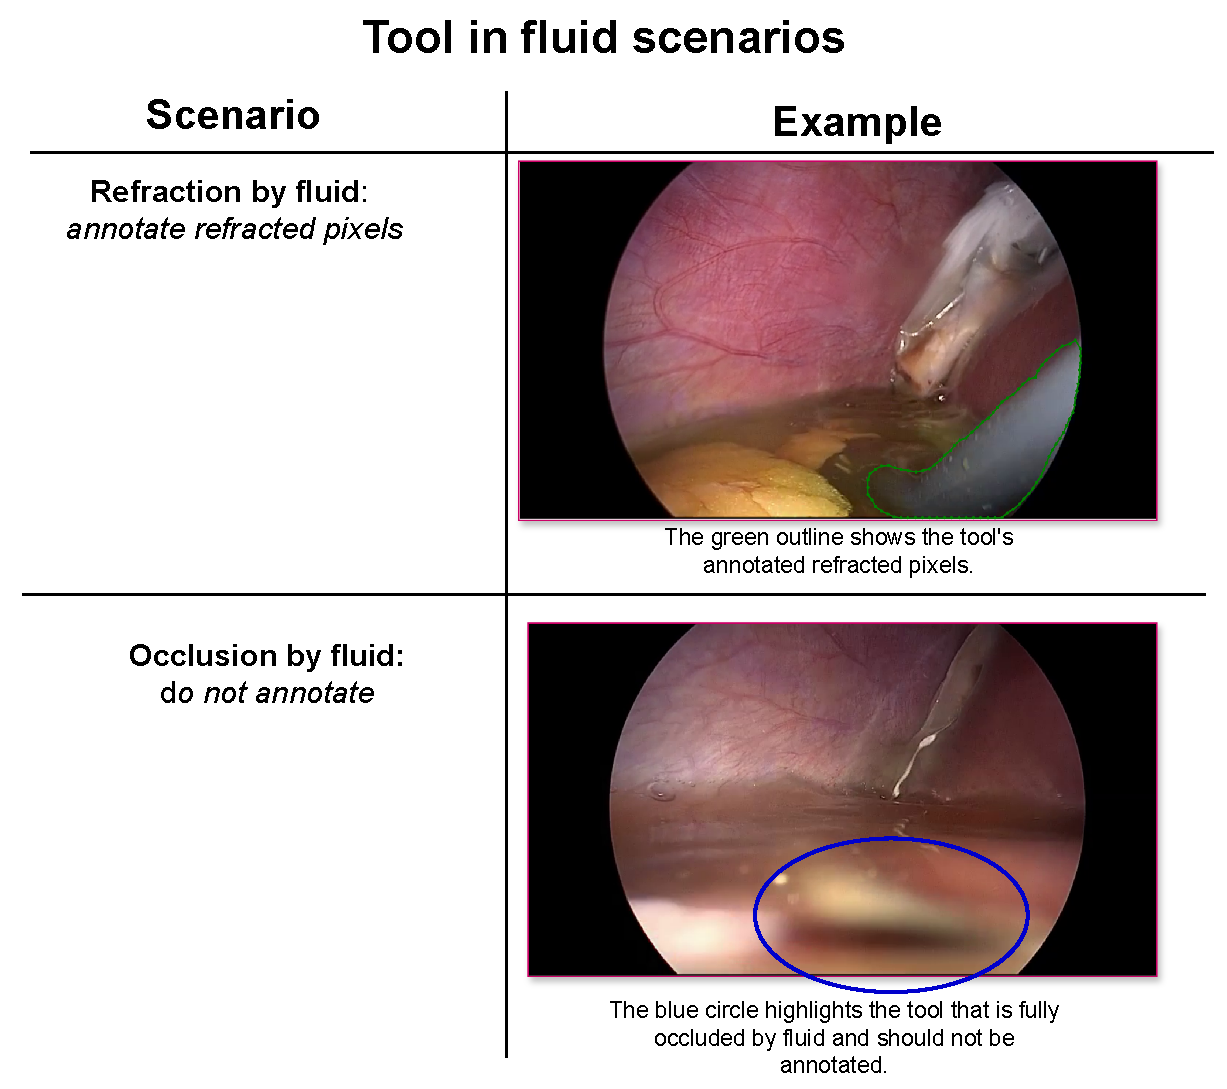
\includegraphics[width=0.9\linewidth,height=0.82\textheight,keepaspectratio]{phd_papers/sources/CholecInstanceSEg Supplementary Materials/imgs/hard_cases_annotating_instrument_in_fluid.pdf}
  \caption{Annotation guidelines for tools in fluid scenarios}
  \label{fig:cis:supp-fluid}
\end{figure}

\begin{figure}[p]
  \centering
  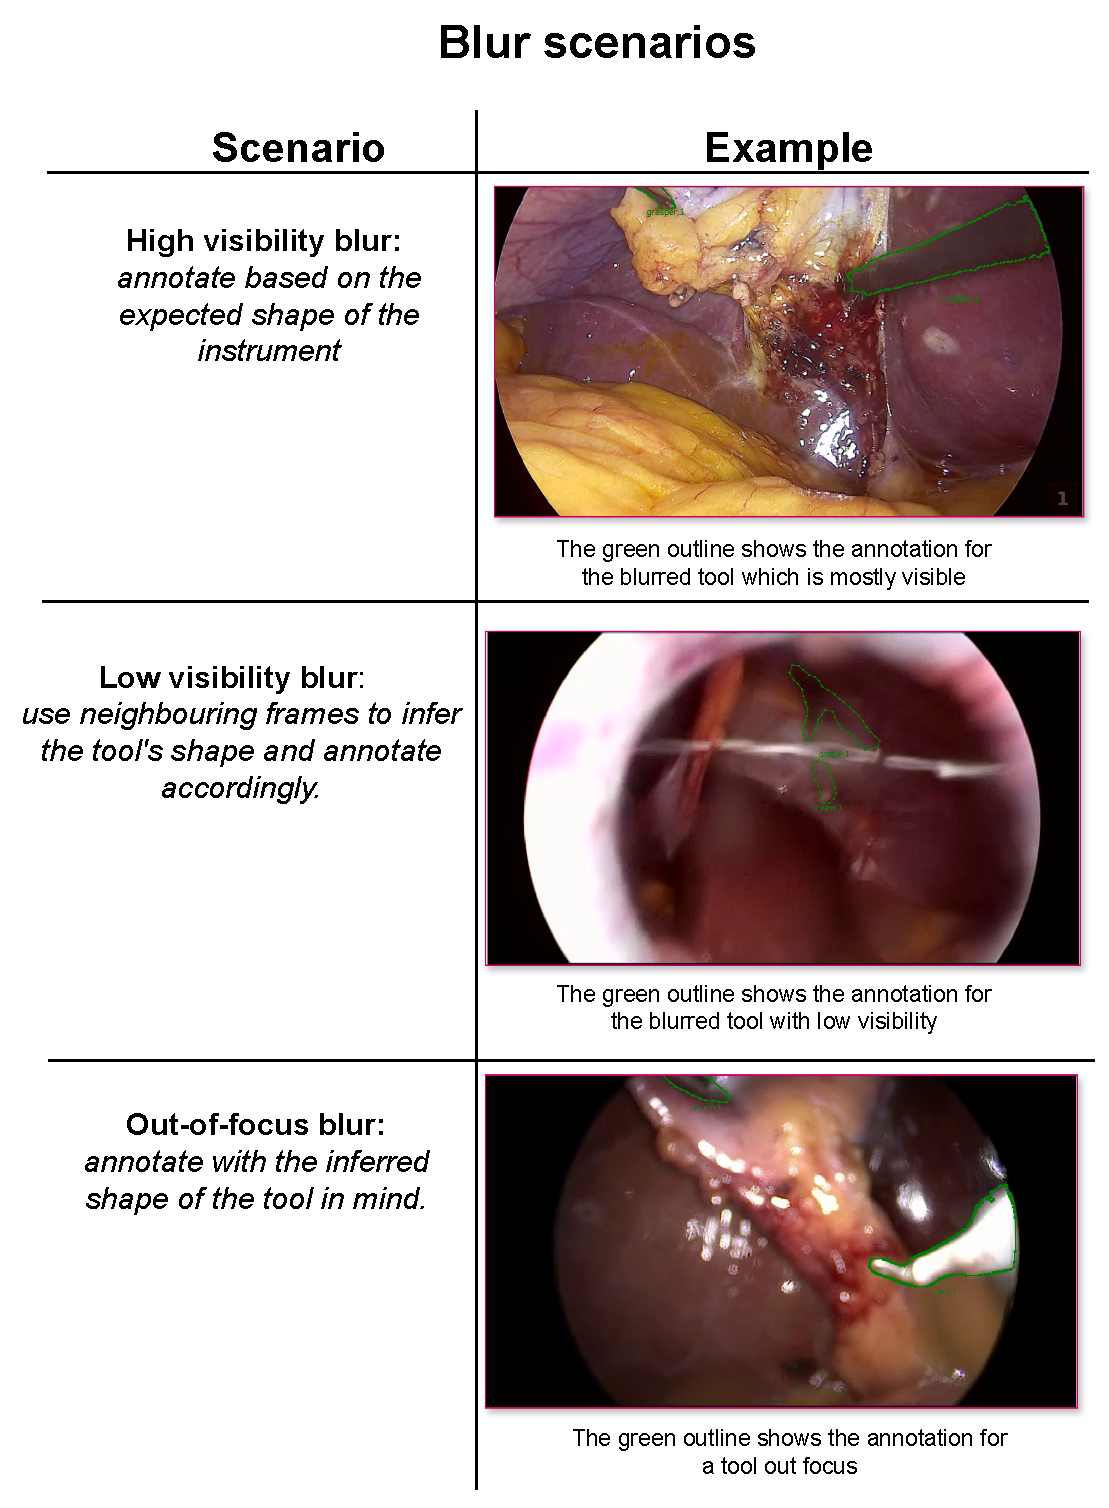
\includegraphics[width=0.9\linewidth,height=0.82\textheight,keepaspectratio]{phd_papers/sources/CholecInstanceSEg Supplementary Materials/imgs/hard_cases_blur.pdf}
  \caption{Annotation guidelines for blur scenarios.}
  \label{fig:cis:supp-blur}
\end{figure}

\begin{figure}[p]
  \centering
  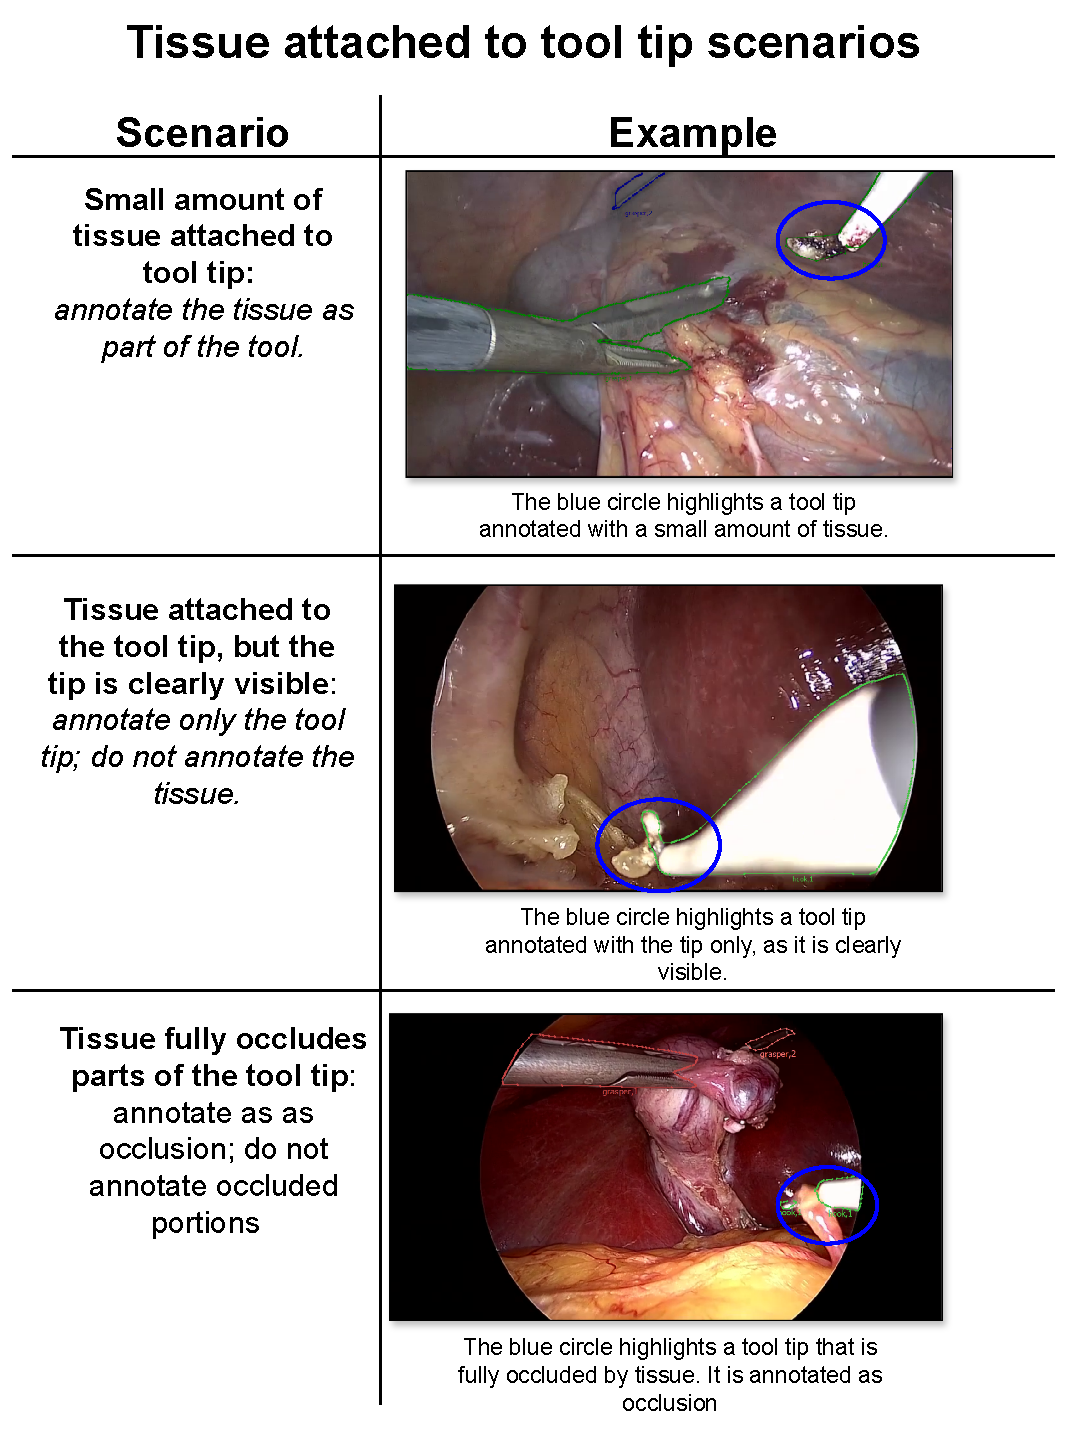
\includegraphics[width=0.9\linewidth,height=0.82\textheight,keepaspectratio]{phd_papers/sources/CholecInstanceSEg Supplementary Materials/imgs/hard_cases_attached_to_instrument.pdf}
  \caption{Annotation guidelines for tissue attached to tool tip scenarios.}
  \label{fig:cis:supp-attached-tissue}
\end{figure}

\begin{figure}[p]
  \centering
  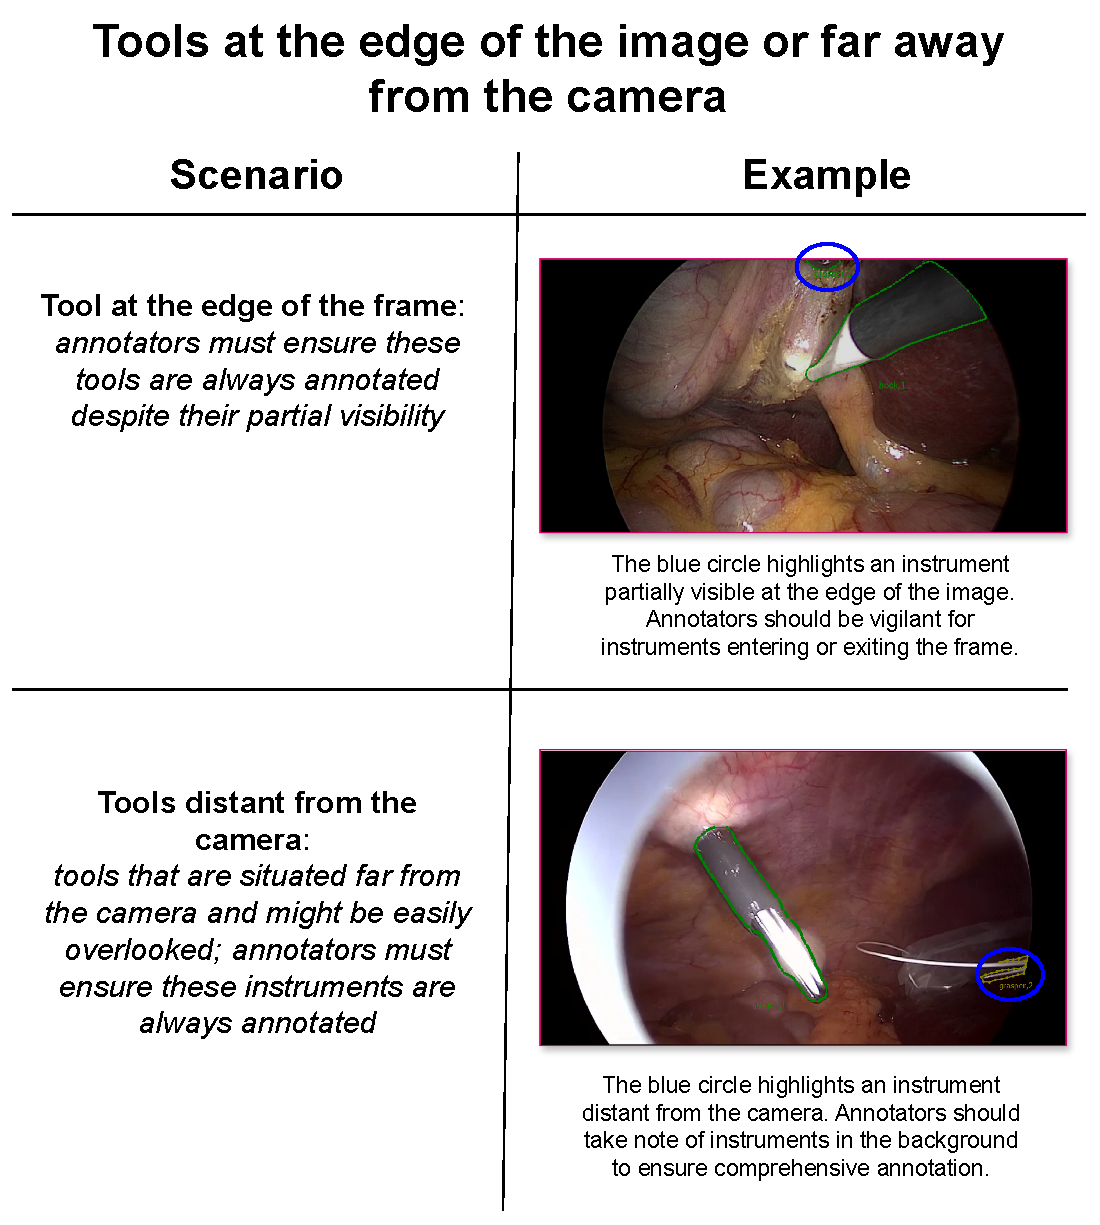
\includegraphics[width=0.9\linewidth,height=0.82\textheight,keepaspectratio]{phd_papers/sources/CholecInstanceSEg Supplementary Materials/imgs/hard_cases_far_and_edge.pdf}
  \caption{Annotation guidelines for instruments at the edge of the frame or distant from the camera.}
  \label{fig:cis:supp-edge-distance}
\end{figure}

\begin{figure}[p]
  \centering
  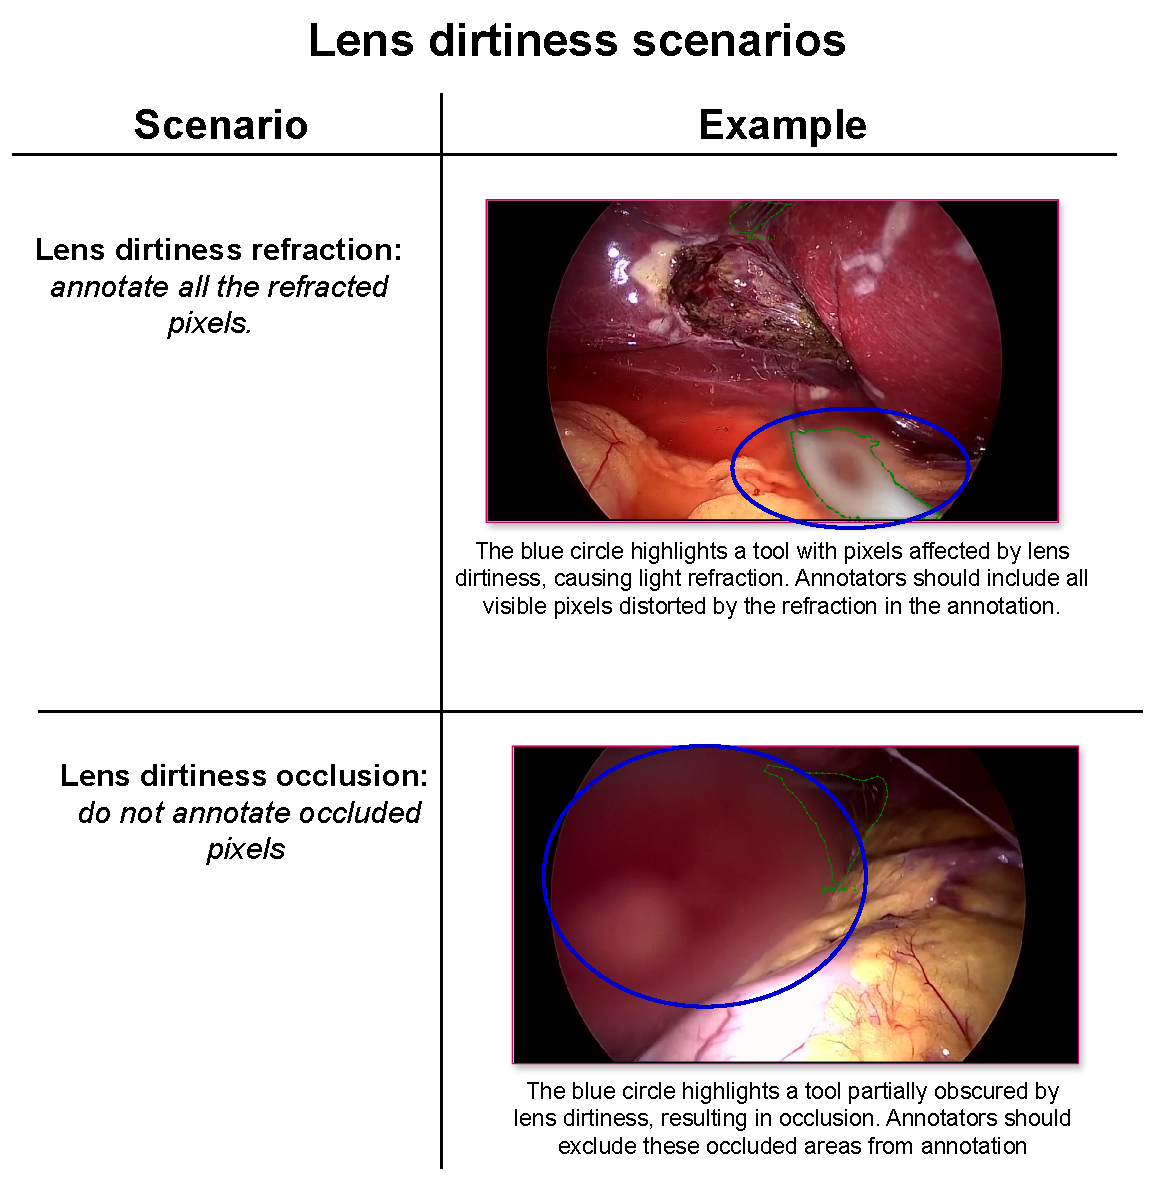
\includegraphics[width=0.9\linewidth,height=0.82\textheight,keepaspectratio]{phd_papers/sources/CholecInstanceSEg Supplementary Materials/imgs/hard_cases_lens_dirtiness.pdf}
  \caption{Annotation guidelines for tools affected by lens dirtiness.}
  \label{fig:cis:supp-lens-dirtiness}
\end{figure}

\begin{figure}[p]
  \centering
  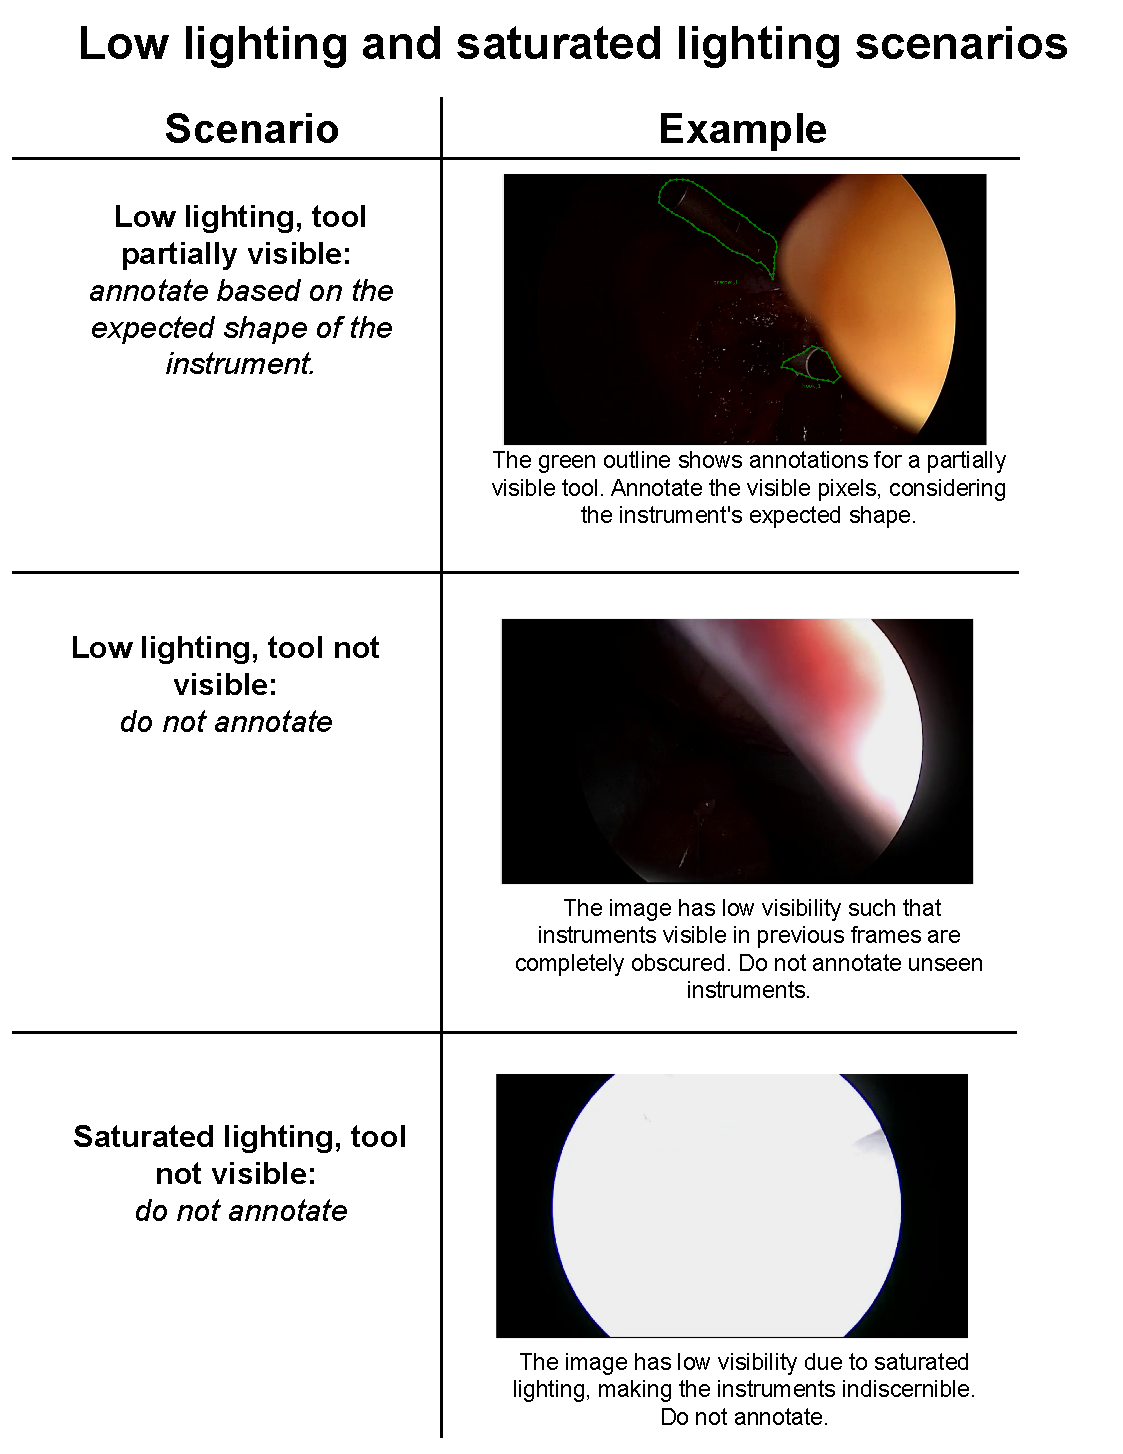
\includegraphics[width=0.9\linewidth,height=0.82\textheight,keepaspectratio]{phd_papers/sources/CholecInstanceSEg Supplementary Materials/imgs/hard_cases_low_lighting_and_bright_lighting.pdf}
  \caption{Annotation guidelines for tools in low lighting and saturated lighting.}
  \label{fig:cis:supp-lighting}
\end{figure}

\begin{figure}[p]
  \centering
  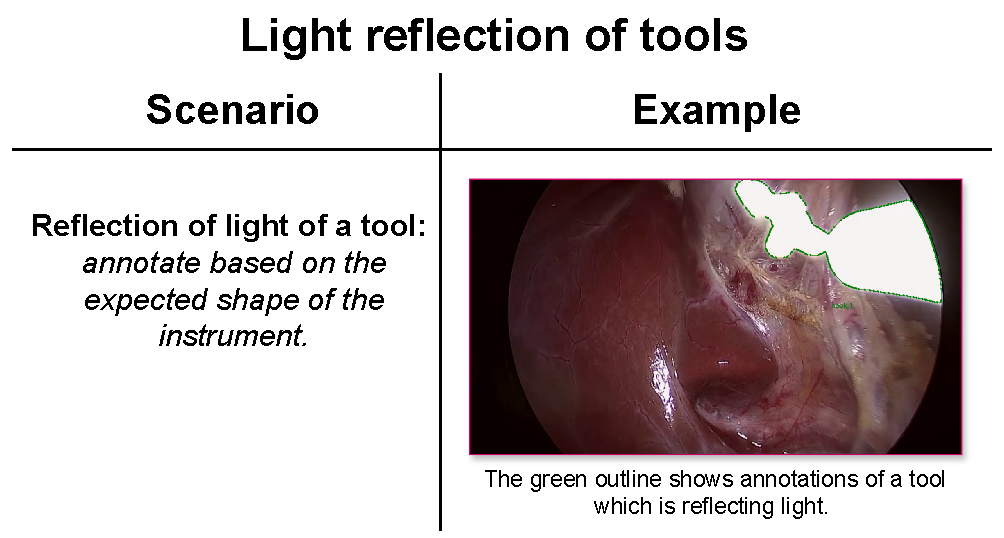
\includegraphics[width=0.9\linewidth,height=0.82\textheight,keepaspectratio]{phd_papers/sources/CholecInstanceSEg Supplementary Materials/imgs/hard_cases_reflection.pdf}
  \caption{Guidelines for annotating tools under light reflection conditions.}
  \label{fig:cis:supp-reflection}
\end{figure}

\begin{figure}[p]
  \centering
  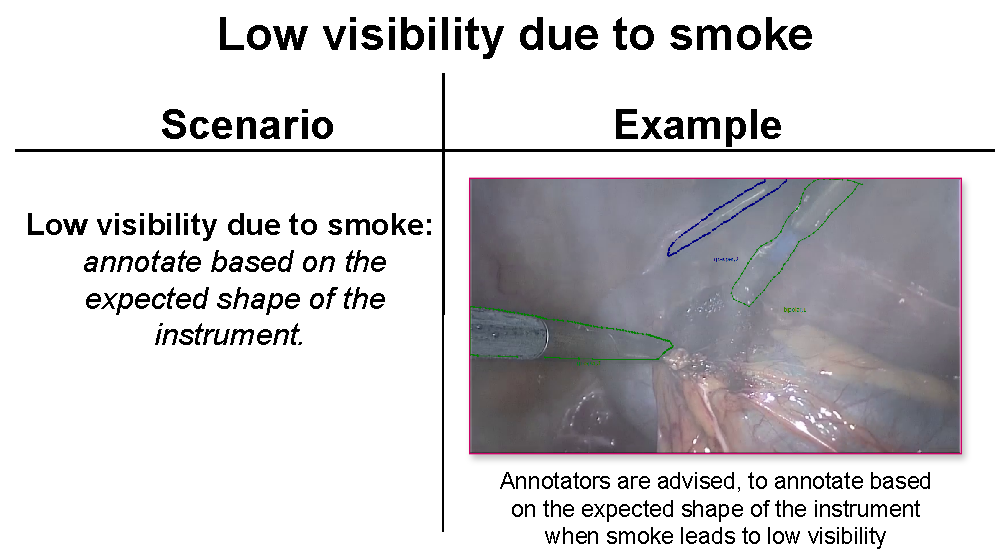
\includegraphics[width=0.9\linewidth,height=0.82\textheight,keepaspectratio]{phd_papers/sources/CholecInstanceSEg Supplementary Materials/imgs/hard_cases_smoke.pdf}
  \caption{Guidelines for annotating tools during low visibility due to smoke.}
  \label{fig:cis:supp-smoke}
\end{figure}

\clearpage
\endgroup
